\begin{enumerate}
\item $ABC$ is a right triangle in which $\angle B = 90\degree$. If $AB = 8 cm$ and $BC = 6 cm$, find the diameter of the circle inscribed in the triangle.

\item Draw two concentric circles of radii $2 cm$ and $5 cm$. Take a point $P$ on the outer circle and construct a pair of tangents $PA$ and $PB$ to the smaller circle. Measure $PA$.  


\item In  \figref{fig:Figh_3}, $PQ$ and $RS$ are two parallel tangents to a circle with centre $O$ and another tangent $AB$ with point of contact $C$ intersecting $PQ$ at $A$ and $RS$ at $B$. Prove that $\angle AOB = 90 \degree$
\begin{figure}[H]
    \centering
    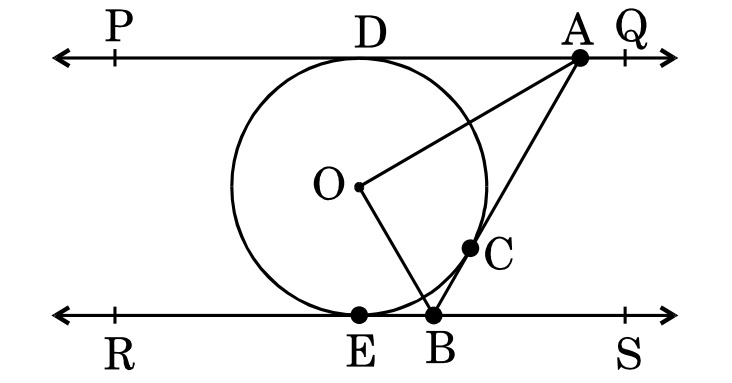
\includegraphics[width=\columnwidth]{figs/img3.jpg}
    \caption{Tangent and Circle}
    \label{fig:Figh_3}
\end{figure}

\item In \figref{fig:Fig-2}, PQ is a chord of length $8 cm$ of a circle of radius $5 cm$. The tangents at $P$ and $Q$ intersect at a point $T$. Find the length $TP$.
\begin{figure}[H]
    \centering
    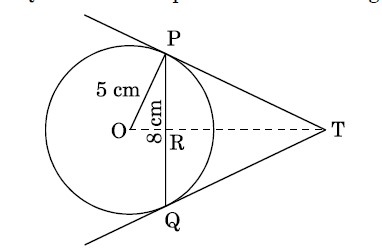
\includegraphics[width=\columnwidth]{figs/Screenshot2023-12-27160239.png}
    \caption{CIRCLE}
    \label{fig:Fig-2}
\end{figure}

\item A chord of a circle of radius $14 cm$ subtends an angle of $60\degree$ at the centre. Find the area of the corresponding minor segment of the circle.
({Use $\hspace{4pt}\pi=\frac{22}{7}$ and $\sqrt{3} = 1.732$})
\item In \figref{fig:circles_456}, $PQ$ is a chord of length $8 cm$ of a circle of radius $5 cm$ and centre $\vec{O}$. The tangents at $P$ and $Q$ intersect at point $T$. Find the length of $TP$.
\begin{figure}[H]                                             \centering
         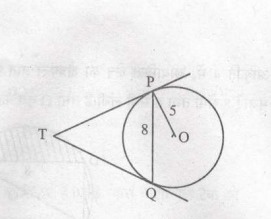
\includegraphics[width=\columnwidth]{figs/i2.jpeg}
			\caption{}
			\label{fig:circles_456}

                \end{figure}
\item Find the area of the segment shown in \figref{fig:circles_768}, if radius of the circle is $21 cm$ and $\angle AOB = 120\degree$ Use $\brak{n =\frac{22}{7}} $
\begin{figure}[H]                                     
\centering
	
 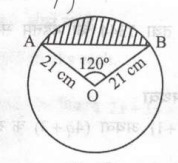
\includegraphics[width=\columnwidth]{figs/img123.jpeg}
		
\caption{cbse}
		
\label{fig:circles_768}
\end{figure}
\item In \figref{fig:circles869}, a circle is inscribed in a $\triangle ABC$ having sides $BC=8 cm$, $AB = 10cm$ and $AC = 12 cm$. Find the lengths $BL$, $CM$ and $AN$.
                                         
\begin{figure}[H]                                     
\centering
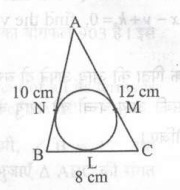
\includegraphics[width=\columnwidth]{figs/img234.jpeg}
\caption{cbse}
\label{fig:circles869}

 \end{figure}
\end{enumerate}
